% Metódy inžinierskej práce

% TODO twoside
\documentclass[10pt,a4paper]{article}

%\usepackage[slovak]{babel}
%\usepackage[T1]{fontenc}
%\usepackage[IL2]{fontenc} % lepšia sadzba písmena Ľ než v T1
\usepackage[utf8]{inputenc}
\usepackage{graphicx}
\usepackage{url} % príkaz \url na formátovanie URL
\usepackage{hyperref} % odkazy v texte budú aktívne (pri niektorých triedach dokumentov spôsobuje posun textu)
\usepackage{lipsum}

\usepackage{cite}
%\usepackage{times}

\pagestyle{headings}

\title{Getting information to the user optimally\thanks{Semestrálny projekt v predmete Metódy inžinierskej práce, ak. rok 2023/24, vedenie: Meno Priezvisko}} % TODO: meno a priezvisko vyučujúceho na cvičeniach

\author{Samuel Tvrdoň\\[2pt]
	{\small Slovenská technická univerzita v Bratislave}\\
	{\small Fakulta informatiky a informačných technológií}\\
	{\small \texttt{...@stuba.sk}}
	}

% TODO:
\date{\small 30. september 2015} % upravte

\begin{document}

\maketitle

\begin{abstract}
% TODO: change a bit
Getting the user, the information they seek as quickly and efficiently as possible is key when talking about searching in today’s world. In this article I am choosing to focus on the ways this is achieved behind the scenes. I want to compare different indexing techniques and other optimizations modern database engines employ to provide optimal storage and retrieval efficiency. I also want to look at methods of making retrieval faster by utilizing caching in a way that increases the performance of storage access. Furthermore, querying the database for data the user wants quickly, would not be possible without proper tokenization of the data in the database, so I would like to mention it as well.
\end{abstract}

\section{Introduction}
% TODO: Add precise paragraph or page cited
\cite{Database-indexing:-yesterday-and-today}
TODO Write about importance of indexing, caching and tokenization

\section{Indexing}


Indexing is used to make querying data faster and more efficient. Since the data can be any size, (TODO: how much data search engines store, https://www.google.com/search/howsearchworks/how-search-works/organizing-information/) and stored in any order, going over every record is unfeasible. With the amount of requests users around the globe make, the equipment costs grow rapidly. To solve this issue, indexing has been introduced as a method to help avoid the need of traversing all of the data on each request.

Indices can be created for each of the parameters that needs to be sorted separately. This reduces storage requirements, drastically. Instead of choosing between searching the table each time and having multiple copies of the table ordered by different columns, a third option is now possible. Storing only references to the real table along with the ordered indices. \ref{fig:index-city}

Another benefit of indices is their reference to the table is only one directional. In other words the table does not care about how many different indices exist, which provides for easy manipulation and flexibility when iterating over database design.

However, indexing isn't one size fits all, there are many options, which cut different corners and make needed optimizations for even faster querying.
\cite{10.1007/978-3-319-93803-5_1}

\begin{figure}
    \centering
    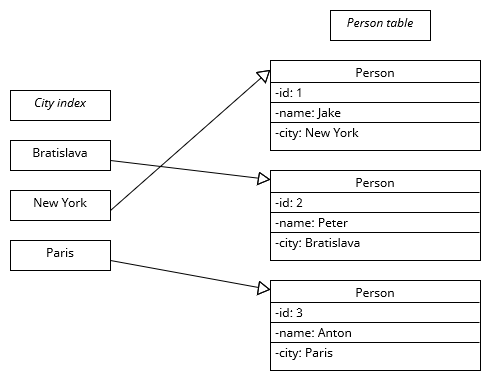
\includegraphics[width=1\linewidth]{Indexing.png}
    \caption{Example of indexing by city name}
    \label{fig:index-city}
\end{figure}

TODO: solarwinds article

TODO: b-trees

\subsection{Composite Index}
https://www.sciencedirect.com/science/article/abs/pii/0164121288900040
\subsubsection{Covering Index}

\section{Caching}
In every system each record is accessed with varying frequency. This fact is leveraged by caching. Caching layer makes for even faster retrieval of the most used records. The most queried records are stored in a temporary memory with faster read speeds than the main larger memory. This helps reduce time as well as the stress on the main storage. \cite{10.1145/3009837.3009891}

\subsection{Caching strategies}

\subsubsection{Cache-aside}
\label{sec:cache-aside}
In this arrangement, users query first requests from the cache. If there is a cache hit, the cache has the requested data and it is returned. If there is a cache miss, the database needs to be queried and the data subsequently returned and stored in the cache for next request. The benefits are in its simplicity and usefulness in general use cases mainly with high read intensity. 
% read-heavy workloads Fit for search engines. 
Cons arise when writing is involved as the speed benefits are lost when any write has to be synced between cache and the database.
% TODO: diagram

\begin{figure}[h]
    \centering
    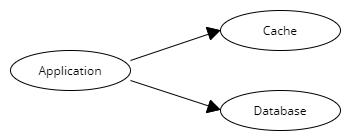
\includegraphics[width=0.5\linewidth]{Cache-aside.png}
    \caption{Cache aside}
    \label{fig:cache-aside}
\end{figure}

% TODO: change to cache through - merge read and write
\subsubsection{Read-through}
Very similiar to Cache-aside \ref{sec:cache-aside} The main difference is in which party is responsible for populating the cache. While in Cache-aside the cache is written to by the application. In Read-through arrangement the cache is hidden behind the database management system. Every request goes through the cache, which then proceeds to call the database.

\subsubsection{Write-through}
Write-through solves the issue of syncing write changes with the cache. In this arrangement all writes as well as reads go through the cache, which, then calls the database. This setup hides the slow main storage away from the users and lets him only talk with the fast cache.

\begin{figure}[h]
    \centering
    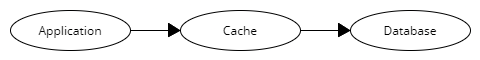
\includegraphics[width=1\linewidth]{Cache-through.png}
    \caption{Cache through}
    \label{fig:cache-through}
\end{figure}

\begin{figure}[h]
    \centering
    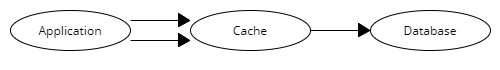
\includegraphics[width=1\linewidth]{Cache-back.png}
    \caption{Cache back}
    \label{fig:cache-back}
\end{figure}

\subsection{Caching algorithms}
Since the cache is way smaller than the main memory. There comes a point when the stored data needs to be cycled. There are various algorithms employed to maximize cache hits and minimize cache misses.

\subsubsection{Random replacement}

\subsubsection{First in first out}

\subsubsection{Least recently used}

\subsubsection{Least frequently used}

\section{Tokenization}


\section{Conclusion}

\newpage

\section*{TODO: References}
\href{https://citeseerx.ist.psu.edu/pdf/24ad3ea19602f0737807cb05fafe44c6c2f86aaf}{Database indexing: yesterday and today}\\
\href{https://dl.acm.org/doi/pdf/10.1145/356643.356645}{HASH TABLE M E T H O D S}\\
\href{https://ieeexplore.ieee.org/abstract/document/755618?casa_token=1dPMFNh1uOMAAAAA:EhTd5TzTa1RHsWQThUec5nDGgAe82xXTYaG32s8GsTNty9qoUoSPlu0Rzh-it8kQ-qtl19_LX-0KjA}{Caching on the World Wide Web}\\
\href{https://link.springer.com/chapter/10.1007/978-981-15-6198-6_18}{Study of Various Methods for Tokenization}\\
\href{https://ieeexplore.ieee.org/abstract/document/1540920?casa_token=hzg5FRuCiVQAAAAA:MDNu1j1gc-DR7xTkOo22jTVIlq55BcYoatyx97bKzY3HdvAw_7-4sRhCNF-iXQcbZQTw2Bb3u0YQxg}{Indexing relational database content offline for efficient keyword-based search}
\href{https://books.google.sk/books?hl=en&lr=&id=yQgfCgAAQBAJ&oi=fnd&pg=PP1&dq=relational+database&ots=qPKwl0TFYt&sig=6jOwNojMeS_JzJYt9NTVB7_gJwk&redir_esc=y#v=onepage&q=relational%20database&f=false}{Relational Database Design and Implementation}


%\acknowledgement{Ak niekomu chcete poďakovať\ldots}

% TODO: add articles
% týmto sa generuje zoznam literatúry z obsahu súboru literatura.bib podľa toho, na čo sa v článku odkazujete
\bibliography{literatura}
\bibliographystyle{abbrv} % prípadne alpha, abbrv alebo hociktorý iný
\end{document}
